\documentclass[12pt]{article}
\usepackage[top=1in, bottom=1in, left=1in, right=1in]{geometry}

\usepackage{setspace}
\onehalfspacing

\usepackage{amssymb}
%% The amsthm package provides extended theorem environments
\usepackage{amsthm}
\usepackage{epsfig}
\usepackage{times}
\renewcommand{\ttdefault}{cmtt}
\usepackage{amsmath}
\usepackage{graphicx} % for graphics files
\usepackage{tabu}

% Draw figures yourself
\usepackage{tikz} 

% writing elements
\usepackage{mhchem}

% The float package HAS to load before hyperref
\usepackage{float} % for psuedocode formatting
\usepackage{xspace}

% from Denovo Methods Manual
\usepackage{mathrsfs}
\usepackage[mathcal]{euscript}
\usepackage{color}
\usepackage{array}

\usepackage[pdftex]{hyperref}
\usepackage[parfill]{parskip}

% math syntax
\newcommand{\nth}{n\ensuremath{^{\text{th}}} }
\newcommand{\ve}[1]{\ensuremath{\mathbf{#1}}}
\newcommand{\Macro}{\ensuremath{\Sigma}}
\newcommand{\rvec}{\ensuremath{\vec{r}}}
\newcommand{\vecr}{\ensuremath{\vec{r}}}
\newcommand{\omvec}{\ensuremath{\hat{\Omega}}}
\newcommand{\vOmega}{\ensuremath{\hat{\Omega}}}
\newcommand{\sigs}{\ensuremath{\Sigma_s(\rvec,E'\rightarrow E,\omvec'\rightarrow\omvec)}}
\newcommand{\el}{\ensuremath{\ell}}
\newcommand{\sigso}{\ensuremath{\Sigma_{s,0}}}
\newcommand{\sigsi}{\ensuremath{\Sigma_{s,1}}}
\newcommand{\ep}{\ensuremath{\varepsilon}}
%---------------------------------------------------------------------------
%---------------------------------------------------------------------------
\begin{document}
\begin{center}
{\bf NE 250, F15\\
November 18, 2015 
}
\end{center}

We've talked about how to discretize energy using the multigroup approximation and angle using $S_N$, $P_N$, or $SP_N$ for the transport equation. \\
This results in a set of ODEs and PDEs with space as the only variable.\\
In this class we're going to talk about options for handling that.
\begin{itemize}
\item ray tracing: this is what we do in Monte Carlo and the integral form of the TE. This allows us to represent ``exact" geometry.
\item There are two ways we can get equation sets with $\nabla^s$ operators: 
  \begin{itemize}
  \item the Diffusion equation. We can apply standard methods for this (learned in 150 I think) or we can apply spherical harmonics in space, which can be manipulated to look a like a bunch of diffusion equations and we handle these as the regular DE.
  \item the even-odd parity TE (which we won't cover). This still has angular dependence but a diffusion-like operator so again we can use the same methods.
  \end{itemize}
\item We will look at the first order form ($\nabla$) here. 
\end{itemize}

\textbf{Spatial Discretization in Slab Geometry} (L\&M 3.3)\\
We'll start by thinking about the 1D, 1-group TE equation that has $S_N$ applied:
\begin{align*}
\mu_n \frac{d \psi_n}{dx} &+ \Sigma_t(x) \psi_n(x) = \sum_{l=0}^L (2l+1) P_l(\mu_n) \Sigma_{s,l}(x) \phi_l(x) + s_n(x)\\
\phi_l(x) &= \frac{1}{2}\sum_{n=1}^N w_n P_l(\mu_n) \psi_n(x)
\end{align*}
%
To deal with the spatial variable we divide space into a grid. The bins do not need to be evenly spaced.\\
We treat cross sections to be constant within each cell, therefore we do well to align bin edges with material boundaries to the degree possible. 
%
\begin{center}
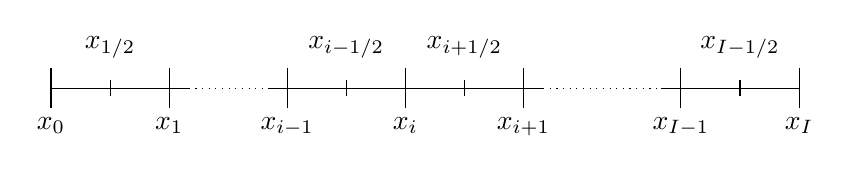
\begin{tikzpicture}
\draw (0,0)--(1.75,0);
\draw (0,-.25)--(0,.25);
\draw (1.5,-.25)--(1.5,.25);
\draw (0.75,-.1)--(0.75,.1);
\draw[dotted] (1.75,0)--(2.75,0);
\draw (2.75,0)--(6.25,0);
\draw[dotted] (6.25,0)--(7.75,0);
\draw (3,-.25)--(3,.25);
\draw (3.75,-.1)--(3.75,.1);
\draw (4.5,-.25)--(4.5,.25);
\draw (5.25,-.1)--(5.25,.1);
\draw (6,-.25)--(6,.25);
\draw (7.75,0)--(9.5,0);
\draw (8,-.25)--(8,.25);
\draw (8.75,-.1)--(8.75,.1);
\draw (9.5, -.25)--(9.5,.25);
\node[below] at (0,-.25) {$x_0$};
\node[above] at (0.75, .25) {$x_{1/2}$};
\node[below] at (1.5,-.25) {$x_1$};
\node[below] at (3,-.25) {$x_{i-1}$};
\node[below] at (4.5,-.25) {$x_i$};
\node[below] at (6,-.25) {$x_{i+1}$};
\node[above] at (3.75, 0.25) {$x_{i-1/2}$};
\node[above] at (5.25, 0.25) {$x_{i+1/2}$};
\node[below] at (8,-.25) {$x_{I-1}$};
\node[above] at (8.75, .25) {$x_{I-1/2}$};
\node[below] at (9.5,-.25) {$x_I$};
\end{tikzpicture}
\end{center}
%
In our derivation we will use both whole points and half points, where half points are halfway between the whole points ($x_{i+1/2} = (1/2)(x_{i+1} - x_{i})$). \\
We also define
\begin{align*}
\Delta_i &= x_{i+1/2} - x_{i-1/2}\\
\Delta_{i-1/2} &= x_{i} - x_{i-1}\\
\Sigma_i &= \Sigma(x) \:, \quad x_{i-1/2} < x < x_{i+1/2}
\end{align*}

We now use this mesh to assign flux values and approximate the derivative term. 


\textbf{sweep pattern and boundary conditions}\\
We solve these equation in the direction of neutron flow. \\
We march through $i = 0, 1, \dots, I$ when $\mu_n > 0$. This is the direction of information transfer and maintains stability of our solution.\\
We march through $i = I, I-1, \dots, 0$ when $\mu_n < 0$ for the same reason.

This marching strategy also informs our boundary conditions. \\
A vacuum boundary condition means no incoming flux. This will be
\begin{align*}
\psi_{0,n}(x) &= 0\:, \quad \mu_n > 0 \quad \text{left vacuum}\\
\psi_{I,n}(x) &= 0\:, \quad \mu_n < 0 \quad \text{right vacuum}
\end{align*}
%
For reflecting, things are a little trickier. We need to map the outgoing flux moving one direction onto the incoming flux coming back the other direction. \\


\textbf{local truncation error}\\




\textbf{Spatial Discretization in Multi-D} (L\&M 4.3)\\
\begin{minipage}{0.5\textwidth}
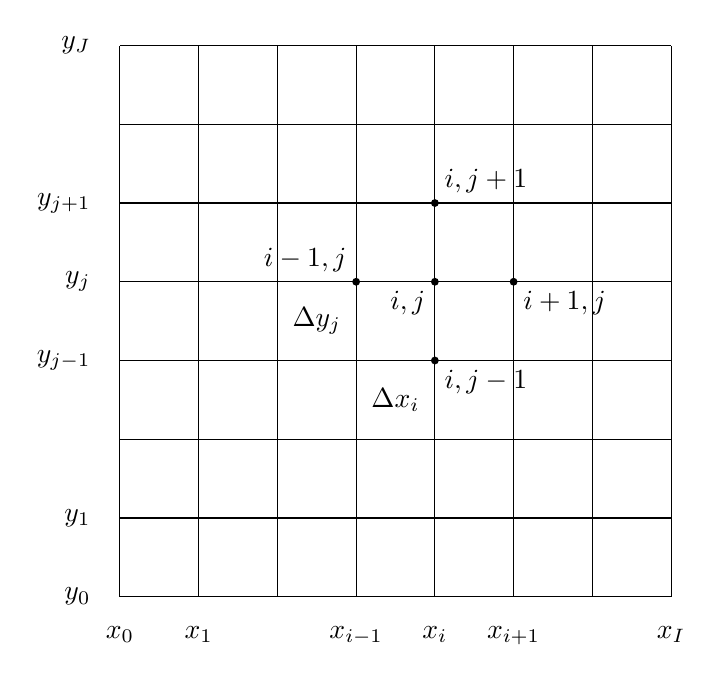
\begin{tikzpicture}
\draw (0,0)--(0,7);
\draw (1,0)--(1,7);
\draw (2,0)--(2,7);
\draw (3,0)--(3,7);
\draw (4,0)--(4,7);
\draw (5,0)--(5,7);
\draw (6,0)--(6,7);
\draw (7,0)--(7,7);
\node[below] at (0,-.25) {$x_0$};
\node[below] at (1,-.25) {$x_1$};
\node[below] at (3,-.25) {$x_{i-1}$};
%\node[above] at (3.5, .25) {$x_{i-1/2}$};
\node[below] at (4,-.25) {$x_i$};
%\node[above] at (4.5, .25) {$x_{i+1/2}$};
\node[below] at (5,-.25) {$x_{i+1}$};
\node[below] at (7,-.25) {$x_I$};
\node at (3.5, 2.5) {$\Delta x_i$};
% begin y
\draw (0,0)--(7,0);
\draw (0,1)--(7,1);
\draw (0,2)--(7,2);
\draw (0,3)--(7,3);
\draw (0,4)--(7,4);
\draw (0,5)--(7,5);
\draw (0,6)--(7,6);
\draw (0,7)--(7,7);
\node[left] at (-.25, 0) {$y_0$};
\node[left] at (-.25,1) {$y_1$};
\node[left] at (-.25,3) {$y_{j-1}$};
\node[left] at (-.25,4) {$y_j$};
\node[left] at (-.25,5) {$y_{j+1}$};
\node[left] at (-.25,7) {$y_J$};
  \node at (2.5,3.5) {$\Delta y_j$};
% labels
\node at (4,4) [circle,fill=black,scale=0.3] {};
\node[below left] at (4,4) {$i,j$};
\node at (5,4) [circle,fill=black,scale=0.3] {};
\node[below right] at (5,4) {$i+1,j$};
\node at (3,4) [circle,fill=black,scale=0.3] {};
\node[above left] at (3,4) {$i-1,j$};
\node at (4,5) [circle,fill=black,scale=0.3] {};
\node[above right] at (4,5) {$i,j+1$};
\node at (4,3) [circle,fill=black,scale=0.3] {};
\node[below right] at (4,3) {$i,j-1$};
\end{tikzpicture}
\end{minipage} \hfill
%
\begin{minipage}{0.5\textwidth}
  \[u(x_i,y_j) = u_{i,j} \qquad u(x_{i+1},y_j) = u_{i+1,j}\]
  \begin{align}
  \frac{\partial^2 u_{i,j}}{\partial x^2} = \frac{\partial}{\partial x}\bigl(\frac{\partial u_{i,j}}{\partial x}\bigr) =
\frac{u_{i-1,j} - 2u_{i,j} + u_{i+1,j}}{\Delta x_i^2} \nonumber \\
%
  \frac{\partial^2 u_{i,j}}{\partial y^2} = \frac{\partial}{\partial y}\bigl(\frac{\partial u_{i,j}}{\partial y}\bigr) =
\frac{u_{i,j-1} - 2u_{i,j} + u_{i,j+1}}{\Delta y_j^2} \nonumber
\end{align}
\end{minipage}

- boundary conditions and sweeping  pattern\\
- quick mention of other spatial methods and their properties


rest of course (3 classes left):\\
- M, 11/23: equation solution procedures (inner iteration, outer iteration, eigenvalue iteration, convergence); one basic solver of each type (SI, GS, PI)\\ 
- M, 11/30: example of research into a different solver for each type (block Krylov, RQI)
- W, 12/02: choice preconditioners? computing architectures? some topic we skipped? Last half of class will be feedback and discussion of class.




\end{document}